\documentclass[14pt]{beamer}
\usepackage{pepslides}
\title{Seismic sources}
\lecturenumber{15}
\hypersetup{pdftitle={Lecture 15: Seismic sources}}

\definecolor{spaceblue}{RGB}{207,226,243}

\begin{document}

\titleslide

\begin{frame}[t]
\heading{From last time\ldots}
Linearised equations of motion:
\begin{eqn}
\rho\frac{\partial^2 u_{i}}{\partial t^2} - \frac{\partial}{\partial x_{j}}\left(A_{ijkl}\frac{\partial u_{k}}{\partial x_{l}}\right) = 0,
\end{eqn}
subject to boundary conditions:
\begin{eqn}
\hat{n}_{j}A_{ijkl}\frac{\partial u_{k}}{\partial x_{l}} = 0.
\end{eqn}
Along with initial conditions on the displacement vector and its time derivative.

\textbf{But where do earthquakes enter into the theory?}
\end{frame}

\begin{frame}
\centering
\includegraphics[height=0.66\paperheight]{ikluft2007_san_andreas_carrizo.jpg}

The San Andreas Fault in the Carrizo Plain of California.
\credit{Ikluft, Wikimedia Commons (CC BY-SA 4.0)}
\end{frame}

\begin{frame}
\centering
\includegraphics[width=0.62\textwidth]{L3F1.pdf}

A schematic cross-section through a thrust fault. You \textbf{don't} need to learn all this terminology.
\end{frame}

\begin{frame}
\centering
\includegraphics[height=0.72\paperheight]{bearphoto1906_san_francisco_street.jpg}

San Francisco, 1906.
\credit{Bear Photo Co., San Francisco (1906)}
\end{frame}

\begin{frame}
\centering
\raisebox{-0.5\height}{\includegraphics[width=0.68\textwidth]{L3F2.pdf}}\hspace{2em}%
\raisebox{-0.5\height}{\includegraphics[height=0.48\paperheight]{gilbert1906_fence_offset.jpg}}\vspace{1.5em}

\textbf{Elastic rebound theory} of Harry Fielding Reid (1859--1944), following the 1906 San Francisco earthquake.
\credit{Photo: G.~K. Gilbert, USGS (1906)}
\end{frame}

\sectionslide{Kinematic source approximation}

\begin{frame}
Lagrangian density for finite elasticity:
\begin{eqn}
\mathcal{L}(\mathbf{x}, t, \bphi, \mathbf{v}, \mathbf{F}) = \frac{1}{2}\rho(\mathbf{x})\|\mathbf{v}\|^2 - W(\mathbf{x}, \mathbf{F}).
\end{eqn}
Motion of the body satisfies \textbf{conservation of energy}:
\begin{eqn}
\begin{gathered}
\frac{\ddns}{\ddns t}\int_{M}E(\mathbf{x}, t)\dd^{3}\mathbf{x} = 0,\\[\eqgap]
E(\mathbf{x}, t) = \frac{1}{2}\rho(\mathbf{x})\|\mathbf{v}(\mathbf{x}, t)\|^2 + W[\mathbf{x}, \mathbf{F}(\mathbf{x}, t)].
\end{gathered}
\end{eqn}
A body in a \textbf{stable} equilibrium configuration will remain in it -- no earthquakes!
\end{frame}

\begin{frame}
To model an earthquake phenomenologically, we break the \textbf{time-translation symmetry}, adding an explicit
time-dependence to the strain energy function:
\begin{eqn}
\mathcal{L}(\mathbf{x}, t, \bphi, \mathbf{v}, \mathbf{F}) = \frac{1}{2}\rho(\mathbf{x})\|\mathbf{v}\|^2 - W(\mathbf{x}, t, \mathbf{F}).
\end{eqn}
Equations of motion are unchanged.

Constitutive equation now has an explicit time-dependence:
\begin{eqn}
T_{ij}(\mathbf{x}, t) = \frac{\partial W}{\partial F_{ij}}[\mathbf{x}, t, \mathbf{F}(\mathbf{x}, t)].
\end{eqn}
\end{frame}

\begin{frame}
We assume that the time-dependent strain energy function can be written:
\begin{eqn}
W(\mathbf{x}, t, \mathbf{F}) = U(\mathbf{x}, \mathbf{C}) - \frac{1}{2}\overline{S}_{ij}(\mathbf{x}, t)C_{ij}.
\end{eqn}
The corresponding first Piola--Kirchhoff stress tensor is:
\begin{eqn}
T_{ij}(\mathbf{x}, t) = F_{ik}(\mathbf{x}, t)\left\{2\frac{\partial U}{\partial C_{kj}}[\mathbf{x}, \mathbf{C}(\mathbf{x}, t)] -
\overline{S}_{kj}(\mathbf{x}, t)\right\}.
\end{eqn}
The first term on the right-hand side is the stress predicted by elasticity, but this differs from the
true stress due to the second term.
\end{frame}

\begin{frame}
The \textbf{stress glut} is defined by:
\begin{eqn}
\begin{aligned}
\overline{T}_{ij}(\mathbf{x}, t) &= F_{ik}(\mathbf{x}, t)\overline{S}_{kj}(\mathbf{x}, t)\\[\eqgap]
&= 2F_{ik}(\mathbf{x}, t)\frac{\partial U}{\partial C_{kj}}[\mathbf{x}, \mathbf{C}(\mathbf{x}, t)] - T_{ij}(\mathbf{x}, t).
\end{aligned}
\end{eqn}
This term quantifies the failure of elasticity to correctly predict stresses in the body.

By definition, the stress glut is \textbf{non-zero} within the \textbf{source region}.

In the full problem, the stress glut would be determined dynamically.

Under the kinematic source approximation, the stress glut is reduced to a parameter.
\end{frame}

\begin{frame}
We add a stress glut as a perturbation to a stress-free equilibrium configuration:
\begin{eqn}
W(\mathbf{x}, t, \mathbf{F}) = U(\mathbf{x}, \mathbf{C}) - \frac{s}{2}\overline{S}_{ij}(\mathbf{x}, t)C_{ij}.
\end{eqn}
Linearisation proceeds almost identically to yield:
\begin{eqn}
\begin{gathered}
\rho\frac{\partial^2 u_{i}}{\partial t^2} - \frac{\partial}{\partial x_{j}}\left(A_{ijkl}\frac{\partial u_{k}}{\partial x_{l}}\right) = -\frac{\partial\overline{S}_{ij}}{\partial x_{j}},\\[\eqgap]
A_{ijkl}\frac{\partial u_{k}}{\partial x_{l}}\hat{n}_{j} = \overline{S}_{ij}\hat{n}_{j}.
\end{gathered}
\end{eqn}
\textbf{Seismic source} associated with an \textbf{effective body force} and \textbf{effective traction} (force
per unit area) on the boundary.
\end{frame}

\sectionslide{Model for an ideal fault}

\begin{frame}
\centering
\includegraphics[height=0.66\paperheight]{L3F3.png}

\textbf{Real faults} involve strong non-elastic deformation across a \textbf{finite fault zone}.
\end{frame}

\begin{frame}
\centering
\begin{tikzpicture}
\node[anchor=south west,inner sep=0pt] (photo) at (0,0) {\includegraphics[height=0.66\paperheight]{L3F3.png}};
\begin{scope}[x={(photo.south east)},y={(photo.north west)}]
  \draw[line width=1.5pt] (0.66,1.03) -- (0.28,-0.02);
  \draw[->,>=stealth,line width=1.5pt] (0.465,0.64) -- (0.375,0.39);
  \draw[->,>=stealth,line width=1.5pt] (0.46,0.36) -- (0.55,0.61);
\end{scope}
\end{tikzpicture}

For an \textbf{ideal fault} we collapse the fault zone to a surface across which \textbf{displacement is discontinuous}.
\end{frame}

\begin{frame}
We consider a \textbf{planar fault} and adapt our coordinates suitably:
\begin{center}
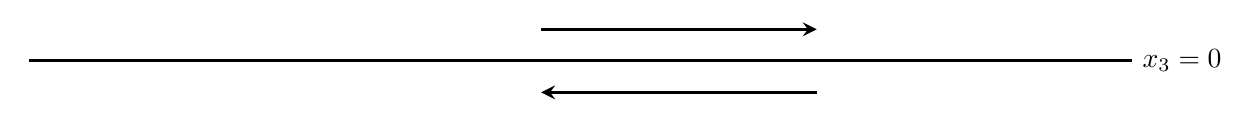
\begin{tikzpicture}
\draw[line width=1.2pt] (0,0) -- (14,0) node[right] {$x_{3}=0$};
\draw[->,>=stealth,line width=1.2pt] (6.5,0.4) -- (10,0.4);
\draw[->,>=stealth,line width=1.2pt] (10,-0.4) -- (6.5,-0.4);
\end{tikzpicture}
\end{center}
Displacement takes the form:
\begin{eqn}
u_{i}(x_1, x_2, x_3, t) = u_{i}^{0}(x_1, x_2, x_3, t) + w_{i}(x_1, x_2, t)H(x_3).
\end{eqn}
The \textbf{displacement discontinuity vector}, $\mathbf{w}$, is tangential to the fault plane ($w_{3}=0$).
\end{frame}

\begin{frame}
Spatial derivative of the displacement vector:
\begin{eqn}
\frac{\partial u_{i}}{\partial x_{j}} = \frac{\partial u_{i}^{0}}{\partial x_{j}} + \frac{\partial w_{i}}{\partial x_{j}}H(x_3) + w_{i}\delta_{j3}\delta(x_3).
\end{eqn}
Resulting linearised stress predicted by elasticity:
\begin{eqn}
A_{ijkl}\frac{\partial u_{k}^{0}}{\partial x_{l}} + A_{ijkl}\frac{\partial w_{k}}{\partial x_{l}}H(x_3) + A_{ijk3}w_{k}\delta(x_3).
\end{eqn}
Motivates the \textbf{definition} of the stress glut:
\begin{eqn}
\overline{S}_{ij} = A_{ijk3}w_{k}\delta(x_3).
\end{eqn}
Simple generalisation to non-planar faults.
\end{frame}

\begin{frame}
Equations of motion with an idealised fault:
\begin{eqn}
\begin{gathered}
\rho\frac{\partial^2 u_{i}}{\partial t^2} - \frac{\partial}{\partial x_{j}}\left(A_{ijkl}\frac{\partial u_{k}}{\partial x_{l}}\right) = -\frac{\partial\overline{S}_{ij}}{\partial x_{j}},\\[\eqgap]
A_{ijkl}\frac{\partial u_{k}}{\partial x_{l}}\hat{n}_{j} = \overline{S}_{ij}\hat{n}_{j},\\[\eqgap]
\overline{S}_{ij} = A_{ijkl}w_{k}\hat{n}_{l}\delta_{\Sigma}.
\end{gathered}
\end{eqn}
Parameters in these equations:
\begin{itemize}
\item Geometry of the earth model
\item Density and the elastic tensor
\item Geometry of the fault plane and the displacement discontinuity vector
\end{itemize}
\end{frame}

\begin{frame}
\centering
\includegraphics[width=0.8\textwidth]{kozdon2013_tohoku_wavefield.jpg}

Numerical simulation of seismic waves generated by rupture on a fault (2011 Tohoku earthquake).
\credit{Kozdon \& Dunham (2013)}
\end{frame}

\sectionslide{Inverse problems}

\begin{frame}
\centering
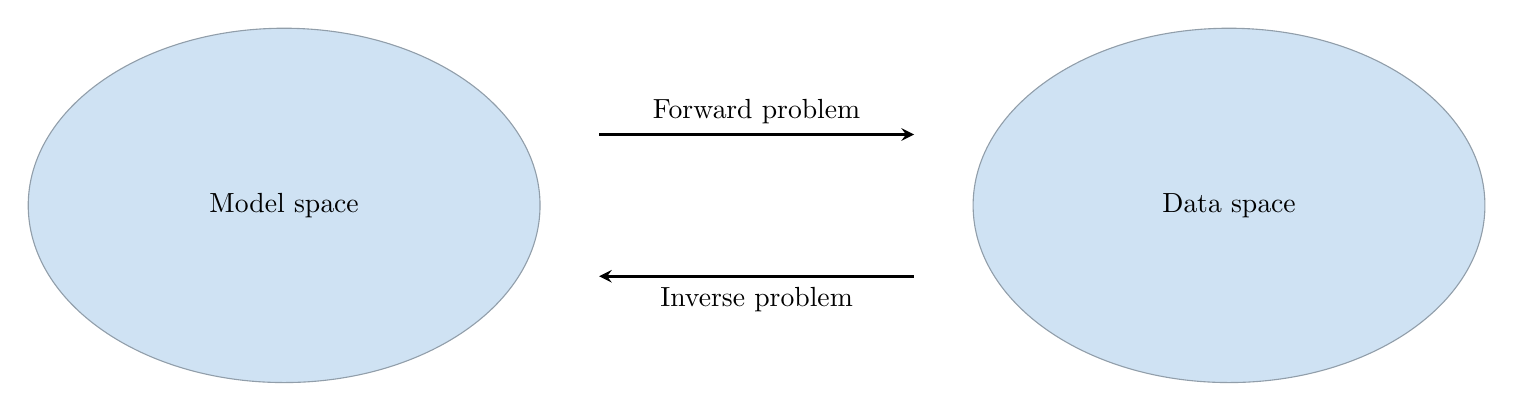
\begin{tikzpicture}[font=\normalsize]
\filldraw[fill=spaceblue,draw=spaceblue!70!black] (0,0) ellipse (3.25 and 2.25);
\filldraw[fill=spaceblue,draw=spaceblue!70!black] (12,0) ellipse (3.25 and 2.25);
\node at (0,0) {Model space};
\node at (12,0) {Data space};
\draw[->,>=stealth,line width=1pt] (4,0.9) -- node[above] {Forward problem} (8,0.9);
\draw[<-,>=stealth,line width=1pt] (4,-0.9) -- node[below] {Inverse problem} (8,-0.9);
\end{tikzpicture}

\vspace{2em}
\raggedright
This graphical representation suggests a \textbf{symmetry} between forward and inverse
problems -- \textbf{this is not the case!}
\end{frame}

\begin{frame}
A mathematical problem can be viewed as a mapping between inputs and outputs.

Such a problem is said to be \textbf{well-posed} if:
\begin{enumerate}
\item For each input there \textbf{exists} an output
\item For each input there exists a \textbf{unique} output
\item The output depends \textbf{continuously} on the input
\end{enumerate}
A problem that is not well-posed is said to be \textbf{ill-posed}.

The equations of mathematical physics are well-posed (or thought/hoped to be).

\textbf{Inverse problems are almost always ill-posed.}
\end{frame}

\begin{frame}[t]
\heading{What you need to know and be able to do}
\begin{enumerate}
\item[(i)] Know that most natural earthquakes are generated by rapid movement across faults within the Earth.
\item[(ii)] Summarise Reid's elastic rebound theory for earthquakes.
\item[(iii)] Explain how a seismic source can be introduced into elasticity using a stress glut, and outline the
derivation of the stress glut for an idealised fault.
\item[(iv)] Understand what is meant by an inverse problem along with the associated terminology and the definition of
well- and ill-posed problems.
\end{enumerate}
\end{frame}

\end{document}
